\begin{figure}[ht]
	\centering
	\includegraphics[width=.80\linewidth]{figures/}
	\caption{}
	\label{fig:}
\end{figure}

simple Table:
\begin{table}[ht]
    \centering
    \begin{tabular}[t]{lcc}
    \toprule
    Layer & $ L_{s} (pH/sq) $ \\
    \midrule
    & \\
    & \\
    & \\
    \bottomrule
    \end{tabular}
    \caption{}
    \label{tab:}
\end{table}%

Highlights:
\hlc[yellow]{Faints.}
\begin{equation}
    \hlmm{\frac{1}{\sqrt{2}}}
\end{equation}

\hlc{It hween the optical and elecrical NEP of a detector as shown in\cite{janssenEquivalenceOpticalElectrical2014} First the theory as stated in the paper will be reviewed and the nessesary mesurements will be discussed. One of the conclusions is that a DC-chip is needed to determine the $T_{c}$ of the Aluminium accurately. Also the quality factor and resonator frequency shift and noise spectra need to be obtained.
}


Tnx this works!
Update nomenclature: 
run in powershell in you top folder the following:
makeindex <filename>.nlo -s nomencl.ist -o <filename>.nls
In which the filename is the name of your main tex file: 
in my case literally: main.tex
so filename = main
makeindex main.nlo -s nomencl.ist -o main.nls

----Paragraph templates----
Simple filled:
%Goal: Title
%Date:__-_ ____
%Grammarly: N

%/Goal: Title
Simple empty:
%Goal: 
%Date:
%Grammarly: N

%/Goal: 
Hamburger empty:
%Top Bun(Topic sentence):
%Date:__-_ ____
%Grammarly: N
%Detail 1:
%Detail 2:
%Detail 3:
%Bottom Bun(Closing sentence):

%/Top Bun(Topic sentence): 
/----Paragraph templates----



\begin{figure}[h!!!!!!!!!!!!!!]
    \centering
    \begin{subfigure}[t]{0.48
    \textwidth}
        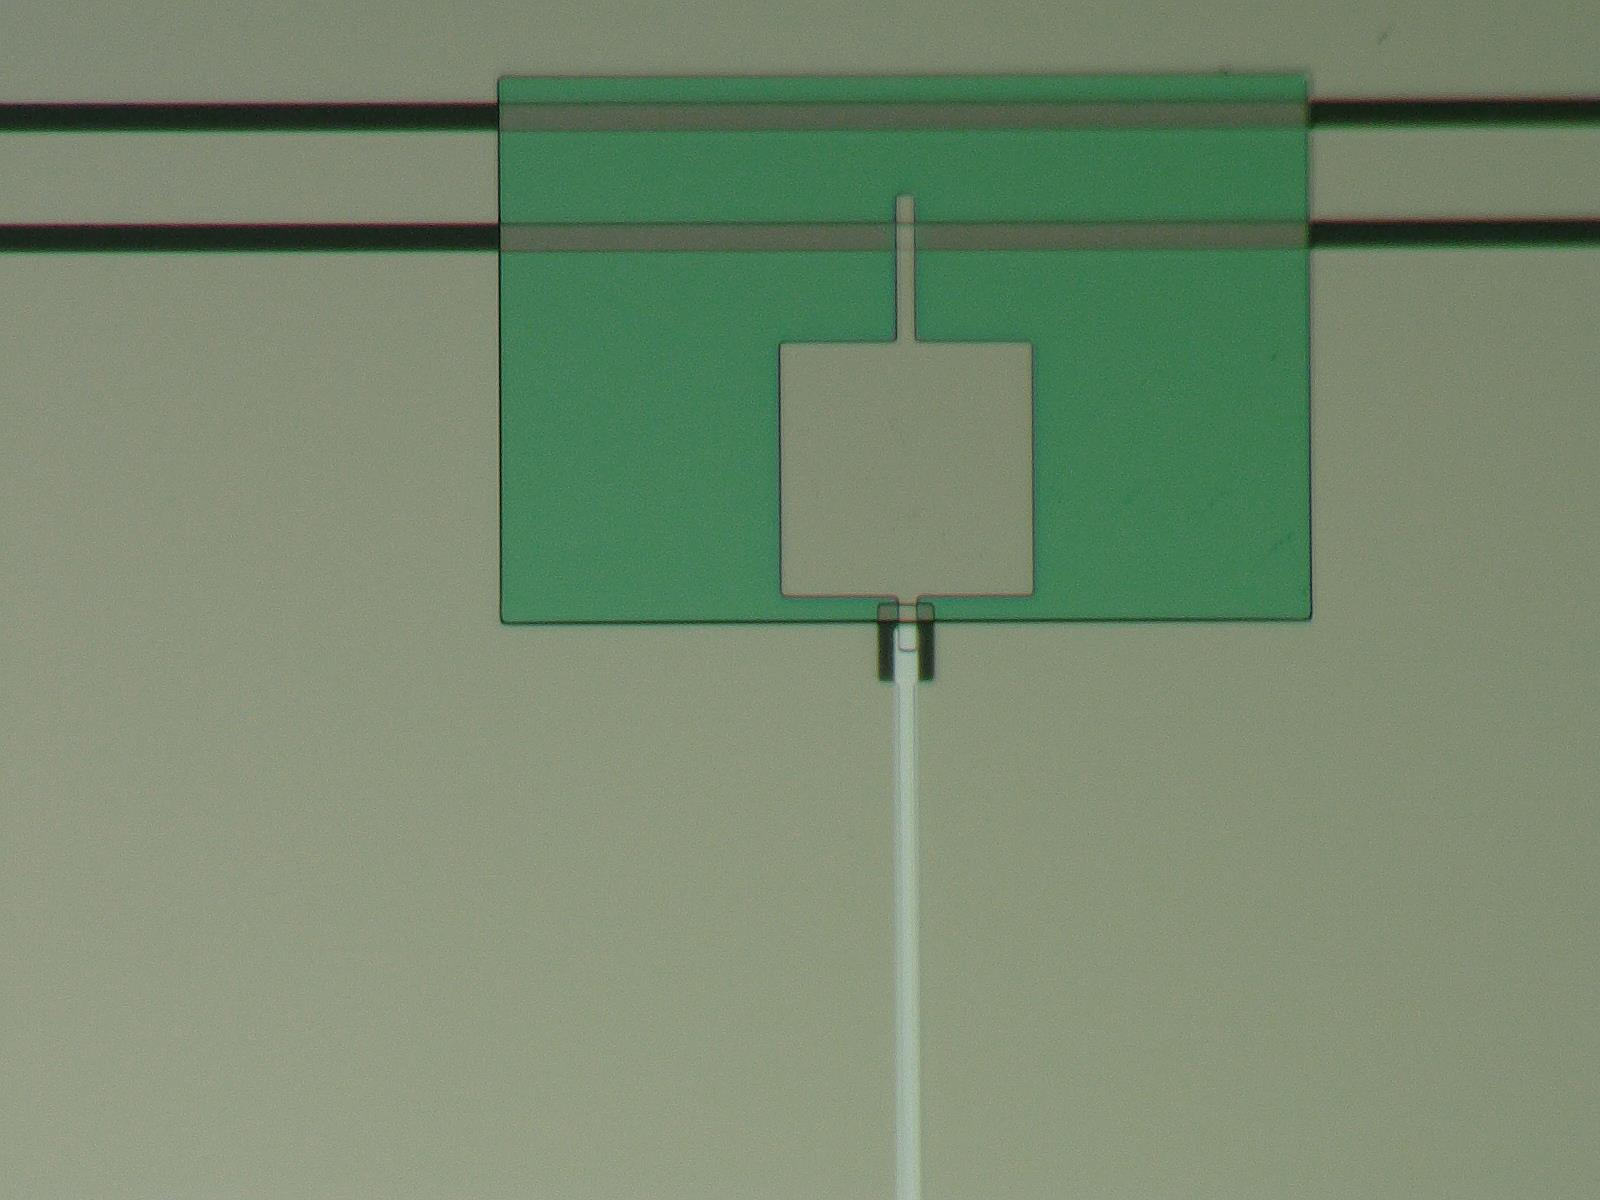
\includegraphics[width=\textwidth]{figures/ch4_design/chip11_19.jpg}
        \caption{}
        \label{fig:ch3_grVStlsgeochange}
    \end{subfigure}
    ~ 
    \begin{subfigure}[t]{0.48\textwidth}
        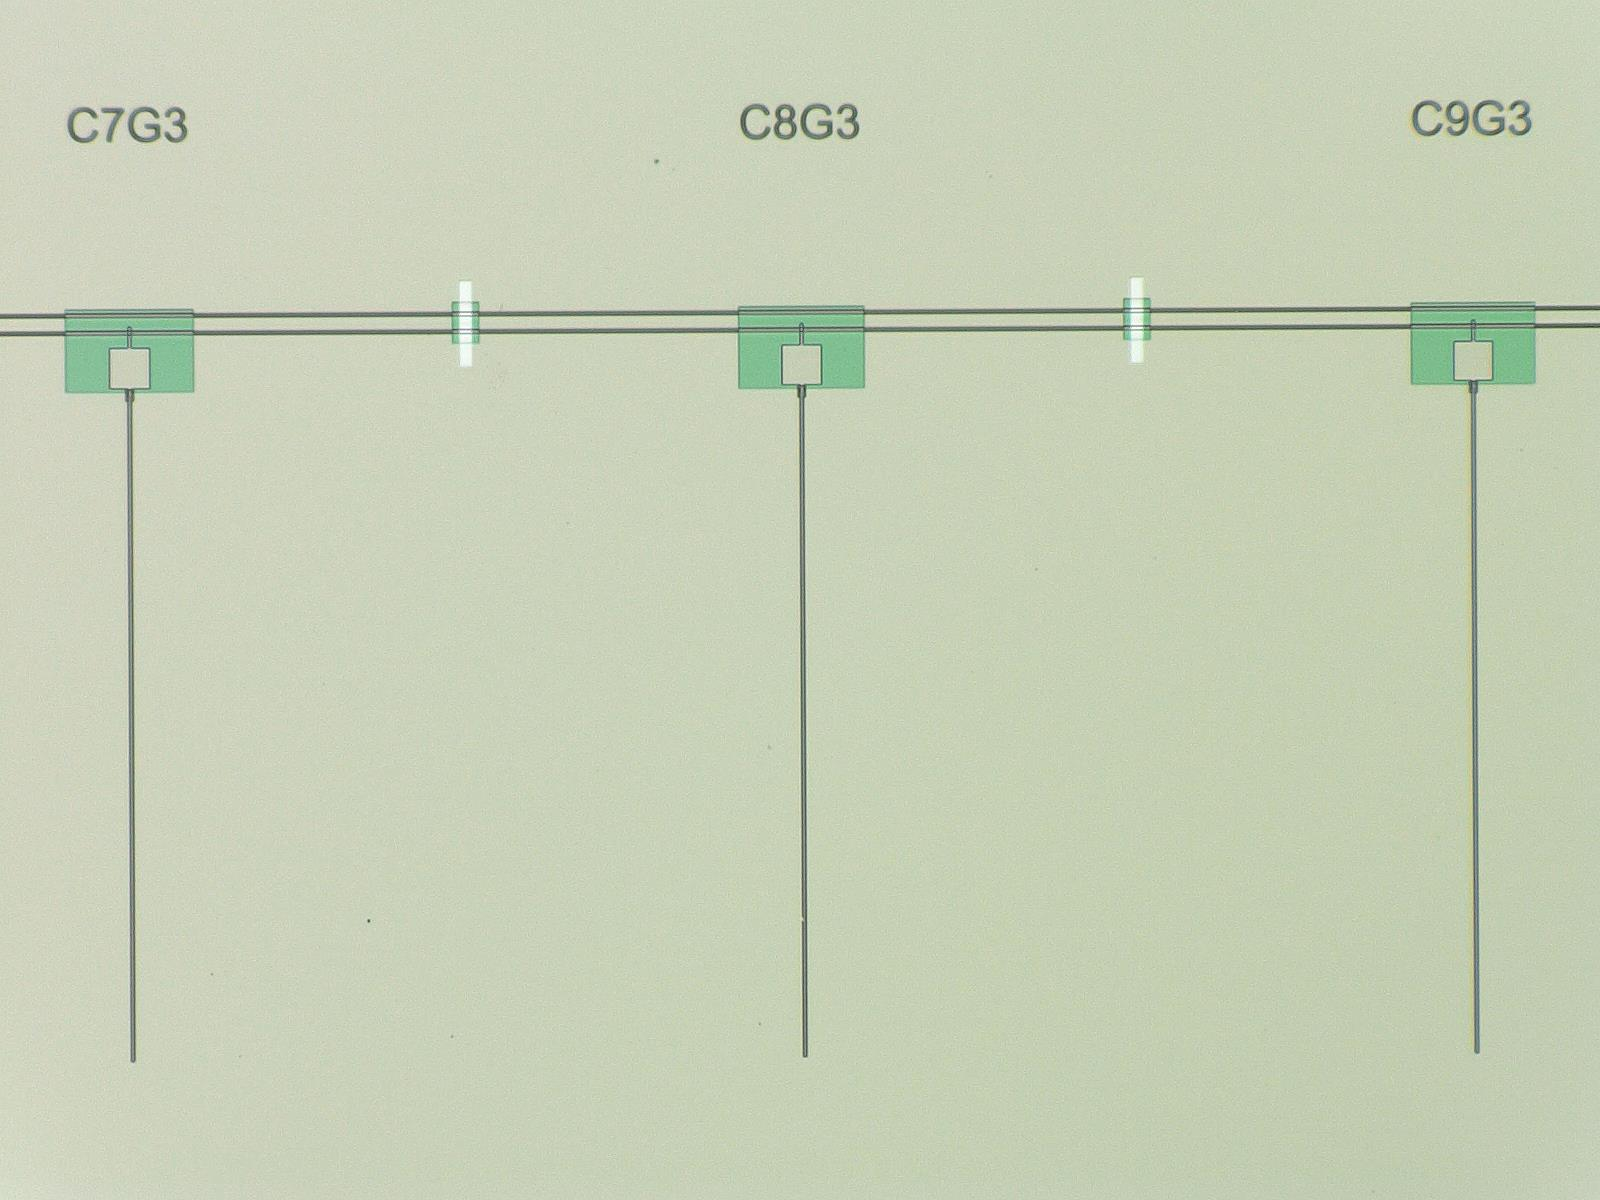
\includegraphics[width=\textwidth]{figures/ch4_design/chip11_20.jpg}
        \caption{}
        \label{fig:ch3_grVStlsreadPchange}
    \end{subfigure}
    \centering
    \begin{subfigure}[t]{0.48
    \textwidth}
        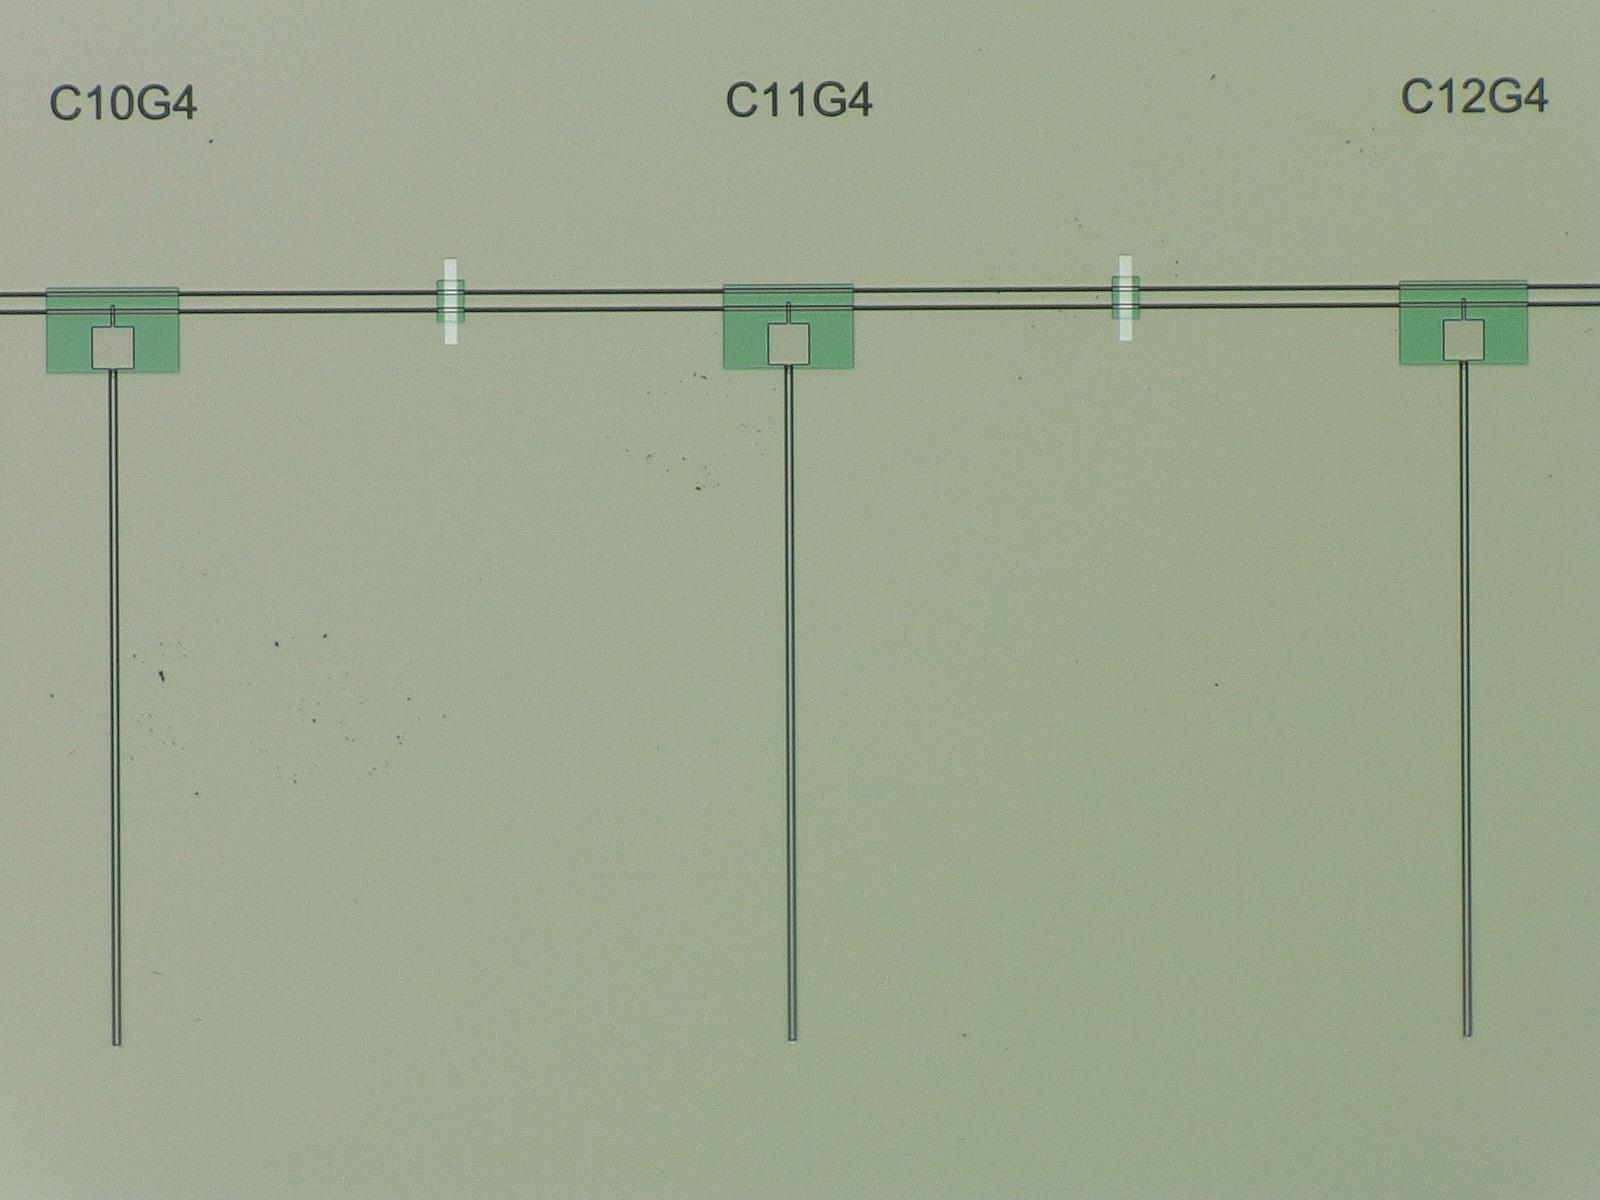
\includegraphics[width=\textwidth]{figures/ch4_design/chip11_21.jpg}
        \caption{}
        \label{fig:ch3_grVStlsgeochange}
    \end{subfigure}
    ~ 
    \begin{subfigure}[t]{0.48\textwidth}
        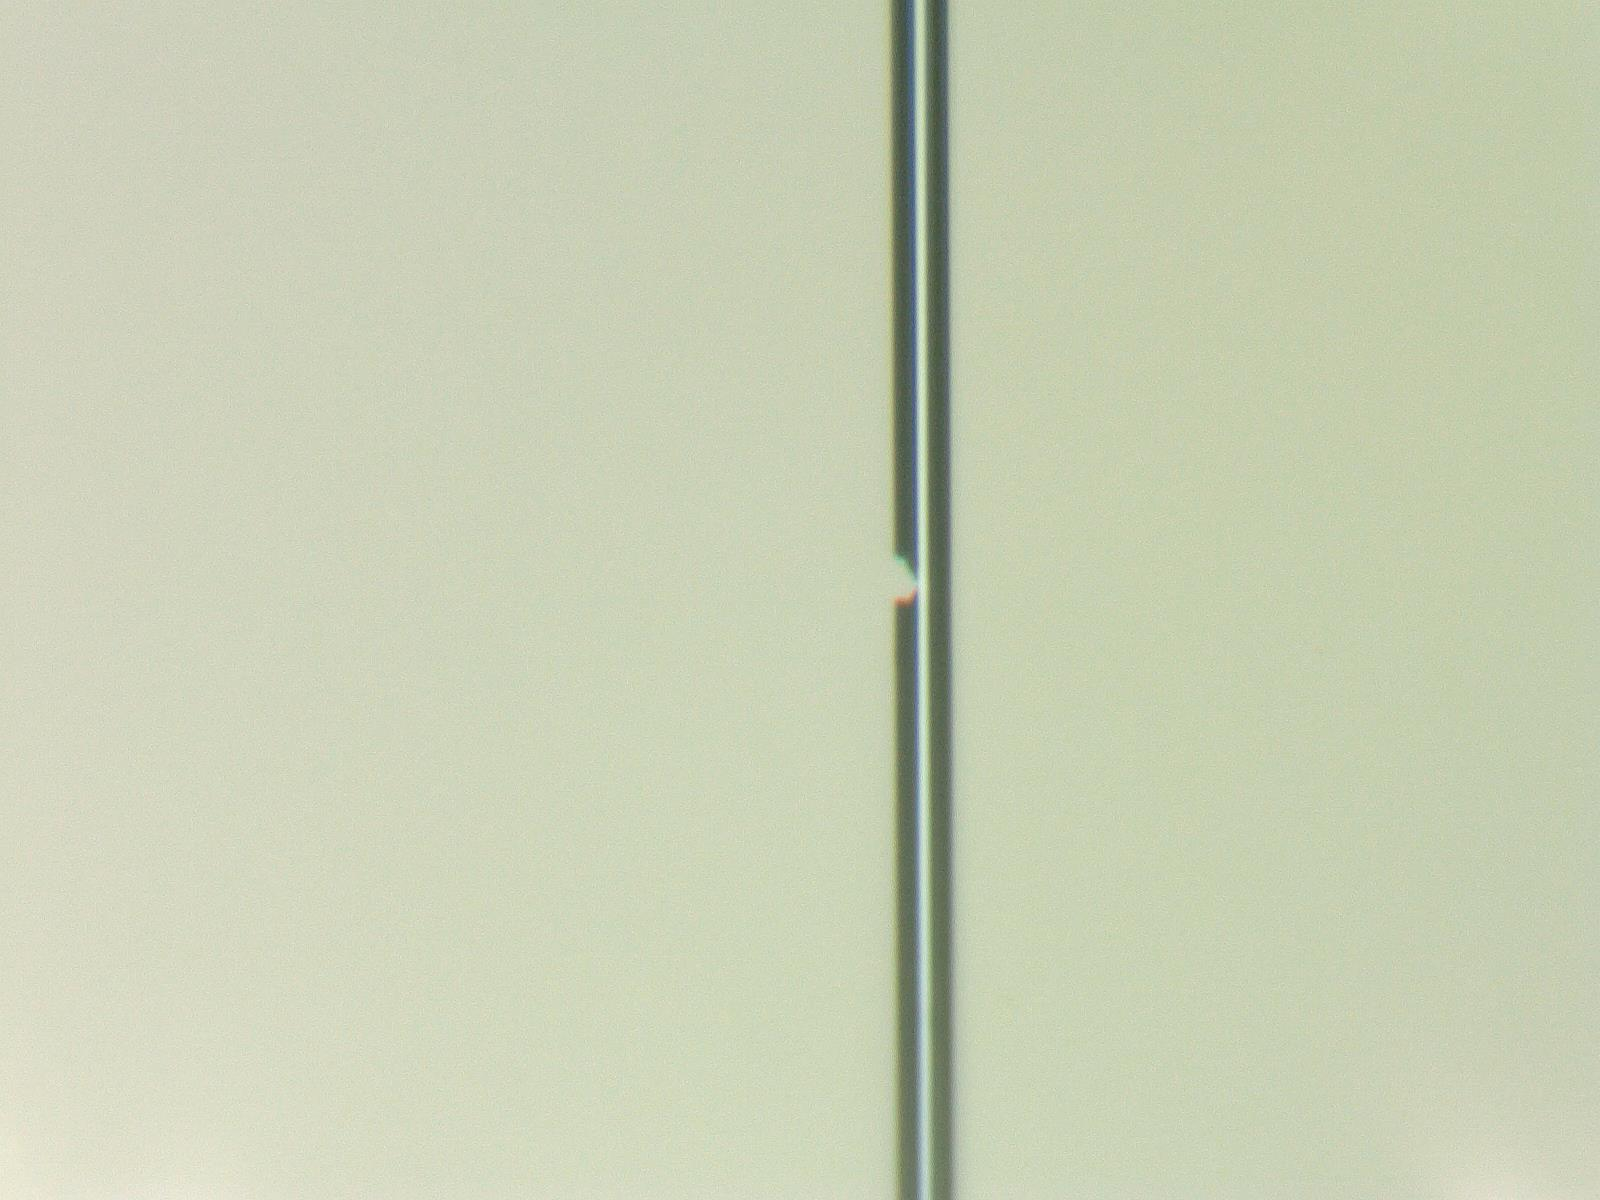
\includegraphics[width=\textwidth]{figures/ch4_design/chip11_G8.jpg}
        \caption{}
        \label{fig:ch3_grVStlsreadPchange}
    \end{subfigure}
    \caption{(a)  (b) (c) (d) }
    \label{fig:AreaVsFreq}
\end{figure}